\addcontentsline{toc}{chapter}{LAMPIRAN}
\titleformat{\section}{\normalfont\bfseries}{\thesection}{1em}{}
% Format judul untuk bagian lampiran
\chapter*{LAMPIRAN}

%\thispagestyle{plain} % Halaman pertama bab menggunakan gaya plain


\newappendix{Lampiran 1. \textit{Layer vision} pada model BLIP}

\begin{figure}[H]
  \centering
  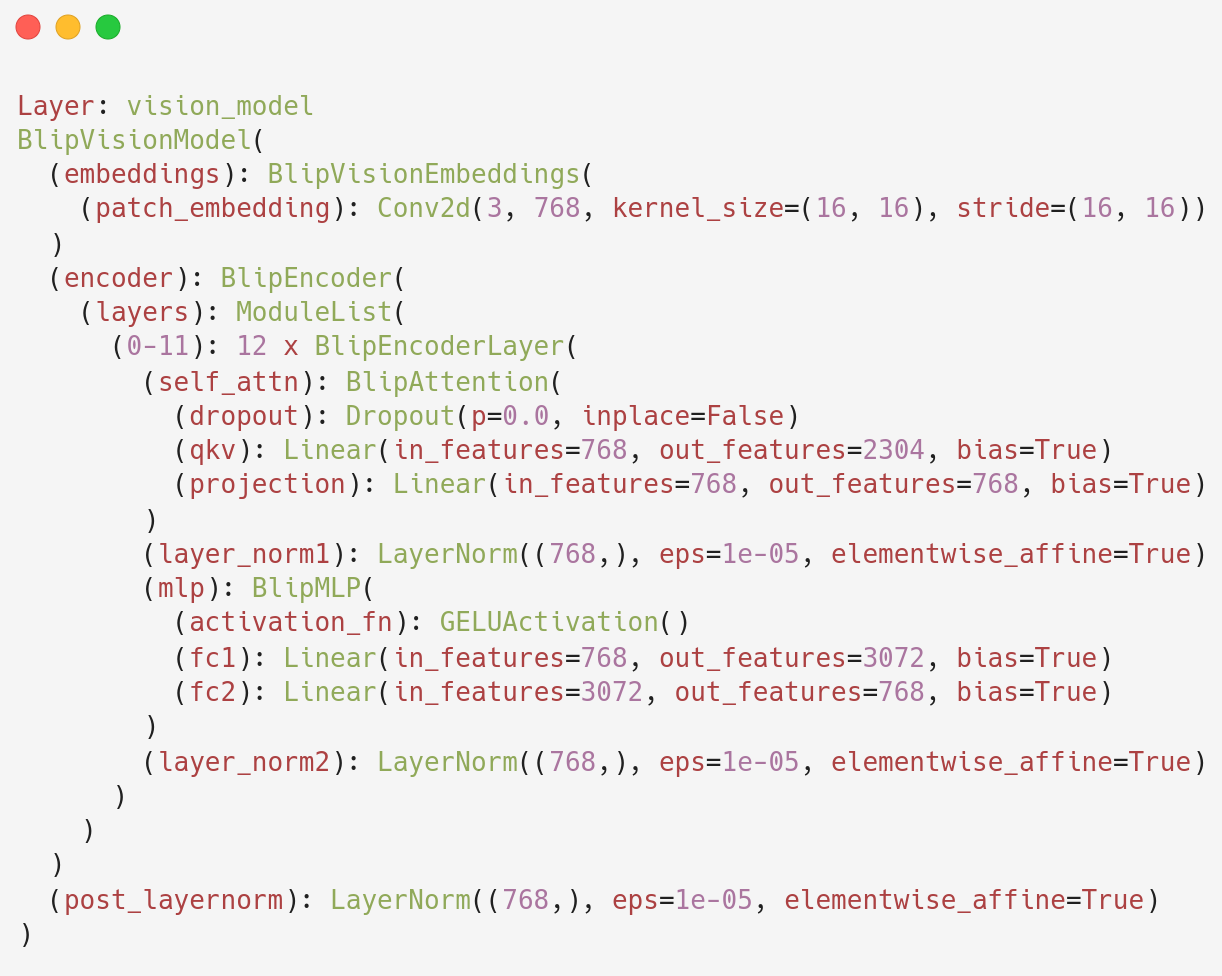
\includegraphics[width=\textwidth, height = 10cm]{image/lampiran/blip-vision-model.png}
  \label{fig:layer-vision-blip}
\end{figure}

\newappendix{Lampiran 2. \textit{Layer text encoder} pada model BLIP}

\begin{figure}[H]
  \centering
  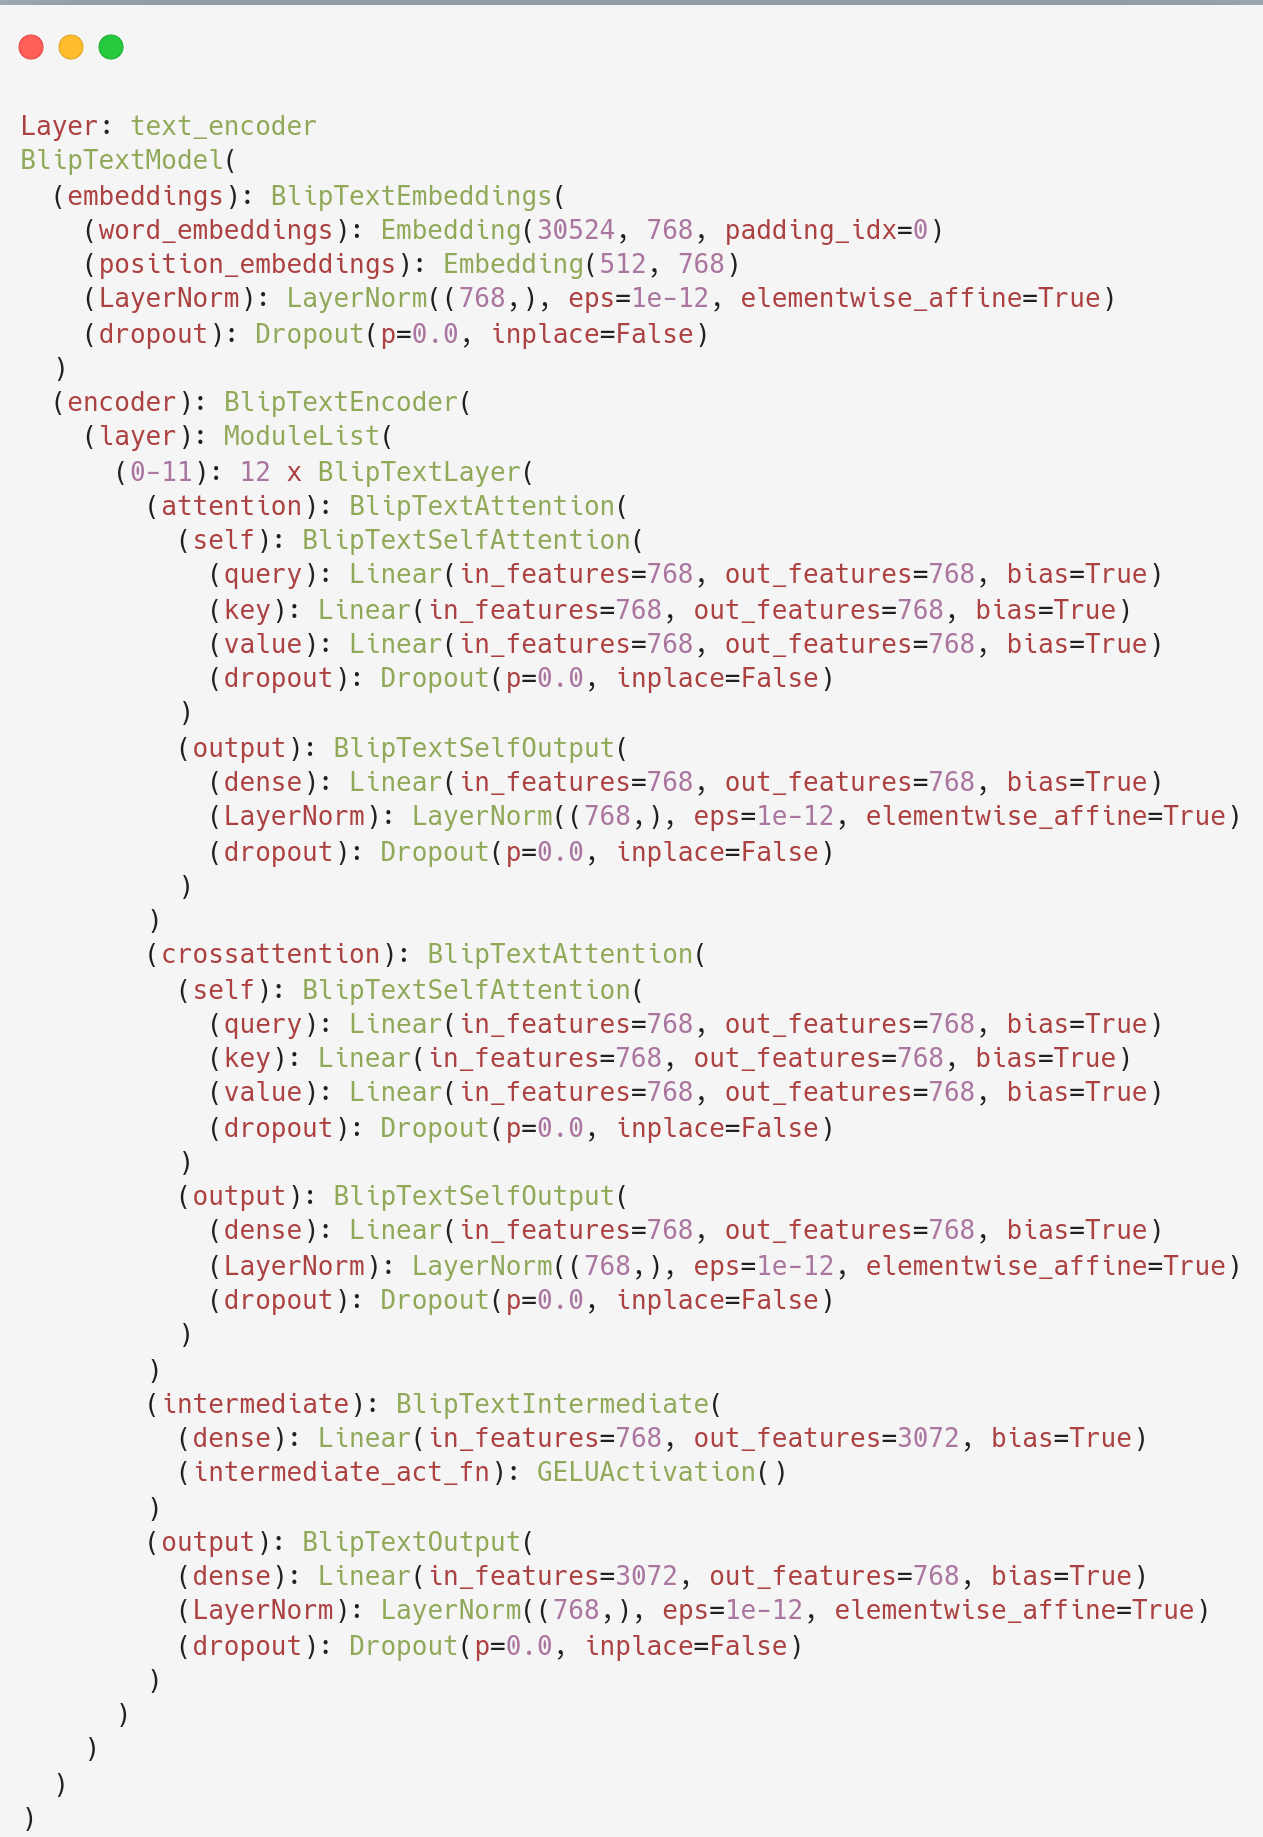
\includegraphics[width=\textwidth]{image/lampiran/blip-text-encoder.png}
  \label{fig:layer-text-encoder-blip}
\end{figure}

\newappendix{Lampiran 3. \textit{Layer text decoder} pada model BLIP}

\begin{figure}[H]
  \centering
  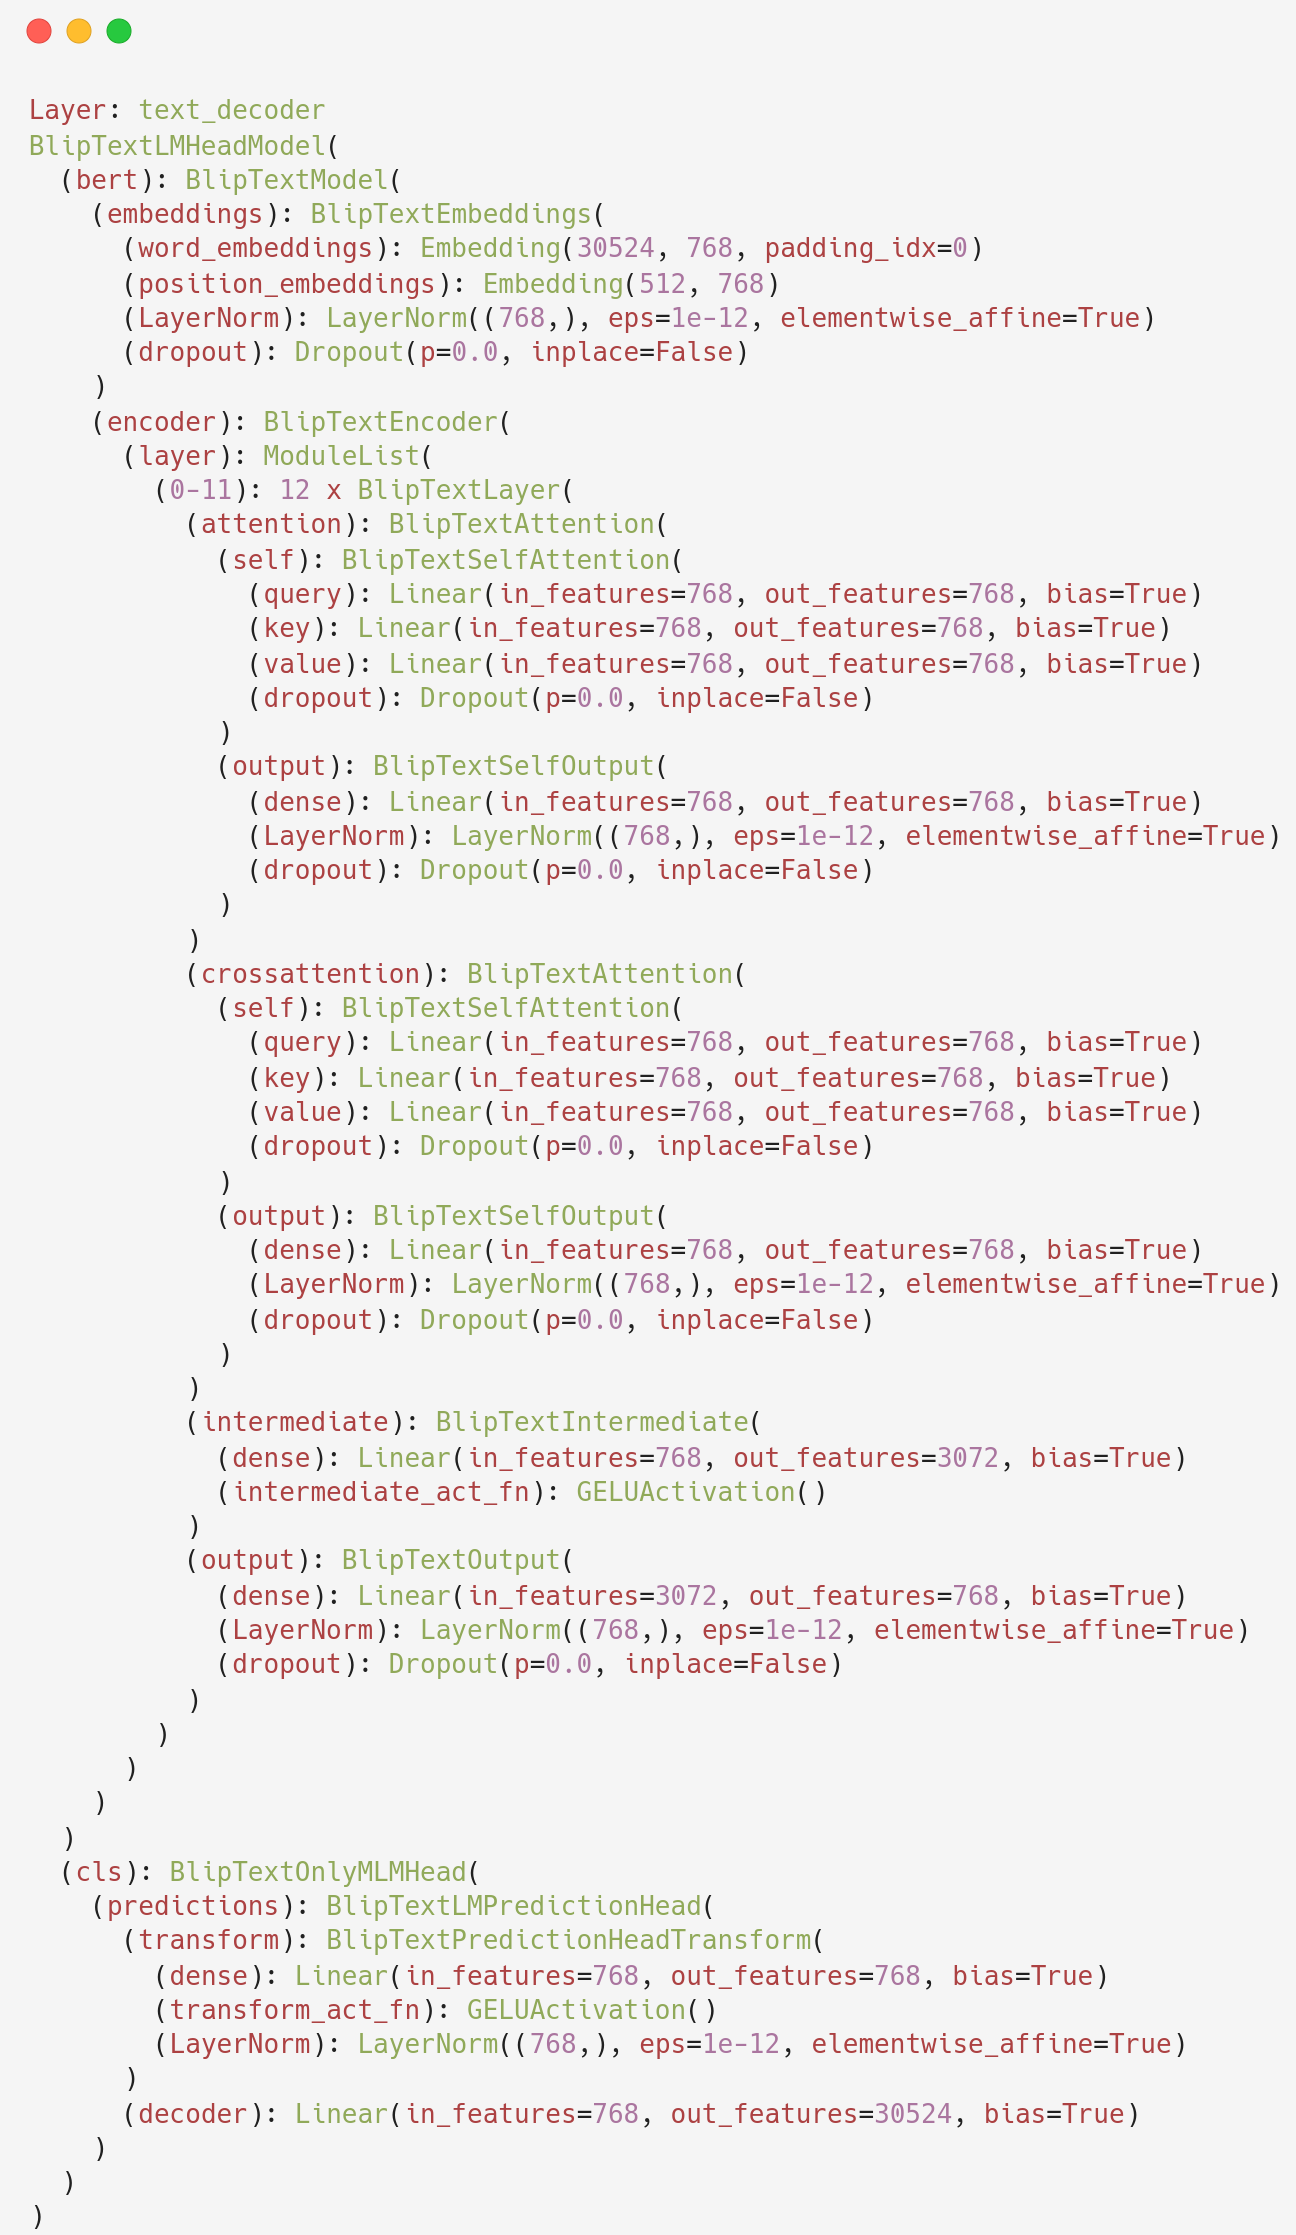
\includegraphics[width=\textwidth, height = 21cm]{image/lampiran/blip-text-decoder.png}
  \label{fig:layer-text-decoder-blip}
\end{figure}


\newappendix{Lampiran 4. Hasil pelatihan dengan VGG19-LSTM untuk pertanyaan \textit{close ended}}

% Please add the following required packages to your document preamble:
% \usepackage{longtable}
% Note: It may be necessary to compile the document several times to get a multi-page table to line up properly
\begin{longtable}[c]{|l|l|l|l|l|l|l|l|}
\hline
\textit{\textbf{Dataset}} &
  \textit{\textbf{Epochs}} &
  \textit{\textbf{\begin{tabular}[c]{@{}l@{}}Batch \\ size\end{tabular}}} &
  \textit{\textbf{\begin{tabular}[c]{@{}l@{}}Learning\\  rate\end{tabular}}} &
  \textbf{Akurasi} &
  \textbf{BLEU-1} &
  \textbf{BLEU-2} &
  \textbf{BLEU-3} \\ \hline
\endfirsthead
%
\endhead
%
PathVQA & 15 & 8  & $1 \times 10^{-5}$ & 43,02\% & 43,02 & 13,60 & 9,41  \\ \hline
PathVQA & 15 & 8  & $5 \times 10^{-5}$ & 53,44\% & 53,45 & 16,90 & 11,69 \\ \hline
PathVQA & 15 & 16 & $1 \times 10^{-5}$ & 44,18\% & 44,18 & 13,97 & 9,67  \\ \hline
PathVQA & 15 & 16 & $5 \times 10^{-5}$ & 51,44\% & 51,44 & 16,27 & 11,25 \\ \hline
PathVQA & 15 & 32 & $1 \times 10^{-5}$ & 47,99\% & 47,99 & 15,18 & 10,50 \\ \hline
PathVQA & 15 & 32 & $5 \times 10^{-5}$ & 45,40\% & 45,40 & 14,36 & 9,93  \\ \hline
PathVQA & 30 & 8  & $1 \times 10^{-5}$ & 39,45\% & 39,45 & 12,48 & 8,63  \\ \hline
PathVQA & 30 & 8  & $5 \times 10^{-5}$ & 48,85\% & 48,85 & 15,45 & 10,69 \\ \hline
PathVQA & 30 & 16 & $1 \times 10^{-5}$ & 52,25\% & 52,25 & 16,52 & 11,43 \\ \hline
PathVQA & 30 & 16 & $5 \times 10^{-5}$ & 49,42\% & 49,42 & 15,63 & 10,81 \\ \hline
PathVQA & 30 & 32 & $1 \times 10^{-5}$ & 38,98\% & 38,98 & 12,33 & 8,53  \\ \hline
PathVQA & 30 & 32 & $5 \times 10^{-5}$ & 49,60\% & 49,60 & 15,69 & 10,85 \\ \hline
PathVQA & 45 & 8  & $1 \times 10^{-5}$ & 48,25\% & 48,25 & 15,26 & 10,56 \\ \hline
PathVQA & 45 & 8  & $5 \times 10^{-5}$ & 48,66\% & 48,66 & 15,39 & 10,65 \\ \hline
PathVQA & 45 & 16 & $1 \times 10^{-5}$ & 38,31\% & 38,32 & 12,12 & 8,39  \\ \hline
PathVQA & 45 & 16 & $5 \times 10^{-5}$ & 51,23\% & 51,24 & 16,20 & 11,21 \\ \hline
PathVQA & 45 & 32 & $1 \times 10^{-5}$ & 49,63\% & 49,65 & 15,70 & 10,86 \\ \hline
PathVQA & 45 & 32 & $5 \times 10^{-5}$ & 14,80\% & 14,80 & 4,68  & 3,24  \\ \hline
VQA-RAD & 15 & 8  & $1 \times 10^{-5}$ & 43,52\% & 43,52 & 13,76 & 9,52  \\ \hline
VQA-RAD & 15 & 8  & $5 \times 10^{-5}$ & 52,85\% & 52,85 & 16,71 & 11,56 \\ \hline
VQA-RAD & 15 & 16 & $1 \times 10^{-5}$ & 47,46\% & 47,46 & 15,01 & 10,38 \\ \hline
VQA-RAD & 15 & 16 & $5 \times 10^{-5}$ & 60,71\% & 60,71 & 19,20 & 13,28 \\ \hline
VQA-RAD & 15 & 32 & $1 \times 10^{-5}$ & 57,27\% & 57,27 & 18,11 & 12,53 \\ \hline
VQA-RAD & 15 & 32 & $5 \times 10^{-5}$ & 62,79\% & 62,79 & 19,86 & 13,74 \\ \hline
VQA-RAD & 30 & 8  & $1 \times 10^{-5}$ & 58,68\% & 58,68 & 18,56 & 12,84 \\ \hline
VQA-RAD & 30 & 8  & $5 \times 10^{-5}$ & 69,05\% & 69,05 & 21,83 & 15,11 \\ \hline
VQA-RAD & 30 & 16 & $1 \times 10^{-5}$ & 60,83\% & 60,83 & 19,24 & 13,31 \\ \hline
VQA-RAD & 30 & 16 & $5 \times 10^{-5}$ & 66,67\% & 66,67 & 21,08 & 14,59 \\ \hline
VQA-RAD & 30 & 32 & $1 \times 10^{-5}$ & 61,02\% & 61,02 & 19,30 & 13,35 \\ \hline
VQA-RAD & 30 & 32 & $5 \times 10^{-5}$ & 57,14\% & 57,14 & 18,07 & 12,50 \\ \hline
VQA-RAD & 45 & 8  & $1 \times 10^{-5}$ & 62,81\% & 62,81 & 19,86 & 13,74 \\ \hline
VQA-RAD & 45 & 8  & $5 \times 10^{-5}$ & 71,05\% & 71,05 & 22,47 & 15,54 \\ \hline
VQA-RAD & 45 & 16 & $1 \times 10^{-5}$ & 57,50\% & 57,50 & 18,18 & 12,58 \\ \hline
VQA-RAD & 45 & 16 & $5 \times 10^{-5}$ & 66,93\% & 66,93 & 21,16 & 14,64 \\ \hline
VQA-RAD & 45 & 32 & $1 \times 10^{-5}$ & 57,98\% & 57,98 & 18,34 & 12,69 \\ \hline
VQA-RAD & 45 & 32 & $5 \times 10^{-5}$ & 68,75\% & 68,75 & 21,74 & 15,04 \\ \hline
\end{longtable}


\newappendix{Lampiran 5. Hasil pelatihan dengan VGG19-LSTM untuk pertanyaan \textit{open ended}}

% Please add the following required packages to your document preamble:
% \usepackage{longtable}
% Note: It may be necessary to compile the document several times to get a multi-page table to line up properly
\begin{longtable}[c]{|l|l|l|l|l|l|l|l|}
  \hline
  \textit{\textbf{Dataset}} &
    \textit{\textbf{Epochs}} &
    \textit{\textbf{\begin{tabular}[c]{@{}l@{}}Batch \\ size\end{tabular}}} &
    \textit{\textbf{\begin{tabular}[c]{@{}l@{}}Learning \\ rate\end{tabular}}} &
    \textbf{Akurasi} &
    \textbf{BLEU-1} &
    \textbf{BLEU-2} &
    \textbf{BLEU-3} \\ \hline
  \endfirsthead
  %
  \endhead
  %
  PathVQA & 15 & 8  & $1 \times 10^{-5}$ & 10,16\% & 10,89 & 3,86  & 2,57  \\ \hline
  PathVQA & 15 & 8  & $5 \times 10^{-5}$ & 19,90\% & 21,41 & 8,01  & 5,38  \\ \hline
  PathVQA & 15 & 16 & $1 \times 10^{-5}$ & 1,29\%  & 1,37  & 0,48  & 0,32  \\ \hline
  PathVQA & 15 & 16 & $5 \times 10^{-5}$ & 18,53\% & 19,95 & 7,96  & 5,23  \\ \hline
  PathVQA & 15 & 32 & $1 \times 10^{-5}$ & 0,43\%  & 0,48  & 0,15  & 0,10  \\ \hline
  PathVQA & 15 & 32 & $5 \times 10^{-5}$ & 15,63\% & 16,67 & 6,25  & 4,01  \\ \hline
  PathVQA & 30 & 8  & $1 \times 10^{-5}$ & 16,17\% & 17,94 & 6,67  & 4,49  \\ \hline
  PathVQA & 30 & 8  & $5 \times 10^{-5}$ & 20,43\% & 22,46 & 9,02  & 5,87  \\ \hline
  PathVQA & 30 & 16 & $1 \times 10^{-5}$ & 14,59\% & 16,22 & 6,49  & 4,29  \\ \hline
  PathVQA & 30 & 16 & $5 \times 10^{-5}$ & 14,48\% & 17,32 & 7,30  & 5,08  \\ \hline
  PathVQA & 30 & 32 & $1 \times 10^{-5}$ & 7,36\%  & 8,01  & 2,83  & 1,88  \\ \hline
  PathVQA & 30 & 32 & $5 \times 10^{-5}$ & 16,49\% & 18,69 & 7,56  & 5,15  \\ \hline
  PathVQA & 45 & 8  & $1 \times 10^{-5}$ & 15,46\% & 18,06 & 7,43  & 5,09  \\ \hline
  PathVQA & 45 & 8  & $5 \times 10^{-5}$ & 22,15\% & 24,28 & 10,02 & 6,81  \\ \hline
  PathVQA & 45 & 16 & $1 \times 10^{-5}$ & 17,61\% & 19,65 & 7,86  & 5,14  \\ \hline
  PathVQA & 45 & 16 & $5 \times 10^{-5}$ & 19,77\% & 22,32 & 9,63  & 6,72  \\ \hline
  PathVQA & 45 & 32 & $1 \times 10^{-5}$ & 13,72\% & 15,74 & 6,51  & 4,31  \\ \hline
  PathVQA & 45 & 32 & $5 \times 10^{-5}$ & 1,95\%  & 2,65  & 1,25  & 0,88  \\ \hline
  VQA-RAD & 15 & 8  & $1 \times 10^{-5}$ & 6,84\%  & 7,87  & 5,53  & 4,27  \\ \hline
  VQA-RAD & 15 & 8  & $5 \times 10^{-5}$ & 15,69\% & 17,60 & 10,74 & 7,37  \\ \hline
  VQA-RAD & 15 & 16 & $1 \times 10^{-5}$ & 5,61\%  & 6,30  & 4,10  & 2,75  \\ \hline
  VQA-RAD & 15 & 16 & $5 \times 10^{-5}$ & 8,85\%  & 10,27 & 7,01  & 4,19  \\ \hline
  VQA-RAD & 15 & 32 & $1 \times 10^{-5}$ & 1,74\%  & 1,90  & 1,90  & 1,44  \\ \hline
  VQA-RAD & 15 & 32 & $5 \times 10^{-5}$ & 5,21\%  & 5,79  & 3,26  & 2,34  \\ \hline
  VQA-RAD & 30 & 8  & $1 \times 10^{-5}$ & 10,58\% & 12,55 & 8,99  & 7,25  \\ \hline
  VQA-RAD & 30 & 8  & $5 \times 10^{-5}$ & 18,18\% & 20,17 & 14,34 & 11,32 \\ \hline
  VQA-RAD & 30 & 16 & $1 \times 10^{-5}$ & 3,81\%  & 5,11  & 3,18  & 2,92  \\ \hline
  VQA-RAD & 30 & 16 & $5 \times 10^{-5}$ & 6,31\%  & 8,17  & 5,68  & 3,91  \\ \hline
  VQA-RAD & 30 & 32 & $1 \times 10^{-5}$ & 5,61\%  & 6,17  & 6,17  & 4,88  \\ \hline
  VQA-RAD & 30 & 32 & $5 \times 10^{-5}$ & 7,96\%  & 9,37  & 6,01  & 4,65  \\ \hline
  VQA-RAD & 45 & 8  & $1 \times 10^{-5}$ & 11,54\% & 12,26 & 7,23  & 5,51  \\ \hline
  VQA-RAD & 45 & 8  & $5 \times 10^{-5}$ & 11,71\% & 13,08 & 7,45  & 4,74  \\ \hline
  VQA-RAD & 45 & 16 & $1 \times 10^{-5}$ & 11,43\% & 13,19 & 10,84 & 6,99  \\ \hline
  VQA-RAD & 45 & 16 & $5 \times 10^{-5}$ & 18,37\% & 20,69 & 16,69 & 11,29 \\ \hline
  VQA-RAD & 45 & 32 & $1 \times 10^{-5}$ & 3,77\%  & 4,97  & 3,80  & 2,97  \\ \hline
  VQA-RAD & 45 & 32 & $5 \times 10^{-5}$ & 14,16\% & 15,16 & 11,64 & 7,85  \\ \hline
  \end{longtable}

\newappendix{Lampiran 6. Hasil pelatihan dengan VGG19-LSTM untuk semua pertanyaan}

% Please add the following required packages to your document preamble:
% \usepackage{longtable}
% Note: It may be necessary to compile the document several times to get a multi-page table to line up properly
\begin{longtable}[c]{|l|l|l|l|l|l|l|l|}
  \hline
  \textit{\textbf{Dataset}} &
    \textit{\textbf{Epochs}} &
    \textit{\textbf{\begin{tabular}[c]{@{}l@{}}Batch \\ size\end{tabular}}} &
    \textit{\textbf{\begin{tabular}[c]{@{}l@{}}Learning \\ rate\end{tabular}}} &
    \textbf{Akurasi} &
    \textbf{BLEU-1} &
    \textbf{BLEU-2} &
    \textbf{BLEU-3} \\ \hline
  \endfirsthead
  %
  \endhead
  %
  PathVQA & 15 & 8  & $1 \times 10^{-5}$ & 26,96\% & 27,32 & 8,84  & 6,07  \\ \hline
  PathVQA & 15 & 8  & $5 \times 10^{-5}$ & 37,07\% & 37,81 & 12,56 & 8,61  \\ \hline
  PathVQA & 15 & 16 & $1 \times 10^{-5}$ & 22,73\% & 22,77 & 7,23  & 4,99  \\ \hline
  PathVQA & 15 & 16 & $5 \times 10^{-5}$ & 34,68\% & 35,41 & 12,04 & 8,19  \\ \hline
  PathVQA & 15 & 32 & $1 \times 10^{-5}$ & 24,39\% & 24,41 & 7,72  & 5,34  \\ \hline
  PathVQA & 15 & 32 & $5 \times 10^{-5}$ & 30,70\% & 31,21 & 10,35 & 7,01  \\ \hline
  PathVQA & 30 & 8  & $1 \times 10^{-5}$ & 27,76\% & 28,65 & 9,56  & 6,55  \\ \hline
  PathVQA & 30 & 8  & $5 \times 10^{-5}$ & 34,41\% & 35,44 & 12,18 & 8,24  \\ \hline
  PathVQA & 30 & 16 & $1 \times 10^{-5}$ & 33,03\% & 33,86 & 11,40 & 7,79  \\ \hline
  PathVQA & 30 & 16 & $5 \times 10^{-5}$ & 31,89\% & 33,32 & 11,45 & 7,94  \\ \hline
  PathVQA & 30 & 32 & $1 \times 10^{-5}$ & 23,19\% & 23,51 & 7,59  & 5,21  \\ \hline
  PathVQA & 30 & 32 & $5 \times 10^{-5}$ & 33,18\% & 34,27 & 11,65 & 8,02  \\ \hline
  PathVQA & 45 & 8  & $1 \times 10^{-5}$ & 31,80\% & 33,11 & 11,33 & 7,82  \\ \hline
  PathVQA & 45 & 8  & $5 \times 10^{-5}$ & 35,20\% & 36,28 & 12,67 & 8,70  \\ \hline
  PathVQA & 45 & 16 & $1 \times 10^{-5}$ & 27,97\% & 28,99 & 9,99  & 6,77  \\ \hline
  PathVQA & 45 & 16 & $5 \times 10^{-5}$ & 35,39\% & 36,67 & 12,89 & 8,95  \\ \hline
  PathVQA & 45 & 32 & $1 \times 10^{-5}$ & 31,43\% & 32,46 & 11,04 & 7,54  \\ \hline
  PathVQA & 45 & 32 & $5 \times 10^{-5}$ & 8,12\%  & 8,48  & 2,90  & 2,01  \\ \hline
  VQA-RAD & 15 & 8  & $1 \times 10^{-5}$ & 24,44\% & 24,98 & 9,48  & 6,79  \\ \hline
  VQA-RAD & 15 & 8  & $5 \times 10^{-5}$ & 36,00\% & 36,87 & 14,00 & 9,66  \\ \hline
  VQA-RAD & 15 & 16 & $1 \times 10^{-5}$ & 27,56\% & 27,89 & 9,82  & 6,75  \\ \hline
  VQA-RAD & 15 & 16 & $5 \times 10^{-5}$ & 34,67\% & 35,38 & 13,08 & 8,71  \\ \hline
  VQA-RAD & 15 & 32 & $1 \times 10^{-5}$ & 28,89\% & 28,97 & 9,83  & 6,86  \\ \hline
  VQA-RAD & 15 & 32 & $5 \times 10^{-5}$ & 38,22\% & 38,47 & 12,77 & 8,87  \\ \hline
  VQA-RAD & 30 & 8  & $1 \times 10^{-5}$ & 36,44\% & 37,36 & 14,13 & 10,26 \\ \hline
  VQA-RAD & 30 & 8  & $5 \times 10^{-5}$ & 46,67\% & 47,54 & 18,54 & 13,44 \\ \hline
  VQA-RAD & 30 & 16 & $1 \times 10^{-5}$ & 34,22\% & 34,83 & 11,74 & 8,46  \\ \hline
  VQA-RAD & 30 & 16 & $5 \times 10^{-5}$ & 36,89\% & 37,81 & 13,48 & 9,32  \\ \hline
  VQA-RAD & 30 & 32 & $1 \times 10^{-5}$ & 34,67\% & 34,94 & 13,06 & 9,32  \\ \hline
  VQA-RAD & 30 & 32 & $5 \times 10^{-5}$ & 32,44\% & 33,15 & 12,01 & 8,56  \\ \hline
  VQA-RAD & 45 & 8  & $1 \times 10^{-5}$ & 39,11\% & 39,45 & 14,03 & 9,94  \\ \hline
  VQA-RAD & 45 & 8  & $5 \times 10^{-5}$ & 41,78\% & 42,45 & 15,06 & 10,21 \\ \hline
  VQA-RAD & 45 & 16 & $1 \times 10^{-5}$ & 36,00\% & 36,82 & 14,76 & 9,97  \\ \hline
  VQA-RAD & 45 & 16 & $5 \times 10^{-5}$ & 45,78\% & 46,79 & 19,22 & 13,18 \\ \hline
  VQA-RAD & 45 & 32 & $1 \times 10^{-5}$ & 32,44\% & 33,01 & 11,49 & 8,11  \\ \hline
  VQA-RAD & 45 & 32 & $5 \times 10^{-5}$ & 41,33\% & 41,83 & 16,67 & 11,43 \\ \hline
  \end{longtable}

\newappendix{Lampiran 7. Hasil pelatihan dengan BLIP untuk pertanyaan \textit{close ended}}

% Please add the following required packages to your document preamble:
% \usepackage{longtable}
% Note: It may be necessary to compile the document several times to get a multi-page table to line up properly
\begin{longtable}[c]{|l|l|l|l|l|l|l|l|}
    \hline
    \textit{\textbf{Dataset}} &
      \textit{\textbf{Epochs}} &
      \textit{\textbf{\begin{tabular}[c]{@{}l@{}}Batch \\ size\end{tabular}}} &
      \textit{\textbf{\begin{tabular}[c]{@{}l@{}}Learning \\ rate\end{tabular}}} &
      \textbf{Akurasi} &
      \textbf{BLEU-1} &
      \textbf{BLEU-2} &
      \textbf{BLEU-3} \\ \hline
    \endfirsthead
    %
    \endhead
    %
    PathVQA & 15 & 8  & $1 \times 10^{-5}$ & 83,44\% & 83,44 & 26,38 & 18,25 \\ \hline
    PathVQA & 15 & 8  & $5 \times 10^{-5}$ & 49,27\% & 49,27 & 15,58 & 10,78 \\ \hline
    PathVQA & 15 & 16 & $1 \times 10^{-5}$ & 72,38\% & 72,38 & 22,89 & 15,83 \\ \hline
    PathVQA & 15 & 16 & $5 \times 10^{-5}$ & 82,85\% & 82,85 & 26,20 & 18,13 \\ \hline
    PathVQA & 15 & 32 & $1 \times 10^{-5}$ & 64,24\% & 64,24 & 20,32 & 14,05 \\ \hline
    PathVQA & 15 & 32 & $5 \times 10^{-5}$ & 79,25\% & 79,25 & 25,06 & 17,34 \\ \hline
    PathVQA & 30 & 8  & $1 \times 10^{-5}$ & 77,15\% & 77,15 & 24,40 & 16,88 \\ \hline
    PathVQA & 30 & 8  & $5 \times 10^{-5}$ & 75,46\% & 75,46 & 23,86 & 16,51 \\ \hline
    PathVQA & 30 & 16 & $1 \times 10^{-5}$ & 74,43\% & 74,43 & 23,54 & 16,28 \\ \hline
    PathVQA & 30 & 16 & $5 \times 10^{-5}$ & 71,00\% & 71,00 & 22,45 & 15,53 \\ \hline
    PathVQA & 30 & 32 & $1 \times 10^{-5}$ & 76,11\% & 76,11 & 24,07 & 16,65 \\ \hline
    PathVQA & 30 & 32 & $5 \times 10^{-5}$ & 86,00\% & 86,00 & 27,20 & 18,82 \\ \hline
    PathVQA & 45 & 8  & $1 \times 10^{-5}$ & 76,02\% & 76,02 & 24,04 & 16,63 \\ \hline
    PathVQA & 45 & 8  & $5 \times 10^{-5}$ & 44,42\% & 44,42 & 14,05 & 9,72  \\ \hline
    PathVQA & 45 & 16 & $1 \times 10^{-5}$ & 77,33\% & 77,33 & 24,45 & 16,92 \\ \hline
    PathVQA & 45 & 16 & $5 \times 10^{-5}$ & 81,77\% & 81,77 & 25,86 & 17,89 \\ \hline
    PathVQA & 45 & 32 & $1 \times 10^{-5}$ & 76,56\% & 76,56 & 24,21 & 16,75 \\ \hline
    PathVQA & 45 & 32 & $5 \times 10^{-5}$ & 81,70\% & 81,70 & 25,83 & 17,87 \\ \hline
    VQA-RAD & 15 & 8  & $1 \times 10^{-5}$ & 61,54\% & 61,54 & 19,46 & 13,46 \\ \hline
    VQA-RAD & 15 & 8  & $5 \times 10^{-5}$ & 56,90\% & 56,90 & 17,99 & 12,45 \\ \hline
    VQA-RAD & 15 & 16 & $1 \times 10^{-5}$ & 0,84\%  & 0,84  & 0,27  & 0,18  \\ \hline
    VQA-RAD & 15 & 16 & $5 \times 10^{-5}$ & 51,24\% & 51,24 & 16,20 & 11,21 \\ \hline
    VQA-RAD & 15 & 32 & $1 \times 10^{-5}$ & 0,90\%  & 0,90  & 0,28  & 0,20  \\ \hline
    VQA-RAD & 15 & 32 & $5 \times 10^{-5}$ & 46,49\% & 46,49 & 14,70 & 10,17 \\ \hline
    VQA-RAD & 30 & 8  & $1 \times 10^{-5}$ & 22,94\% & 22,94 & 7,25  & 5,02  \\ \hline
    VQA-RAD & 30 & 8  & $5 \times 10^{-5}$ & 52,85\% & 52,85 & 16,71 & 11,56 \\ \hline
    VQA-RAD & 30 & 16 & $1 \times 10^{-5}$ & 9,35\%  & 9,35  & 2,96  & 2,04  \\ \hline
    VQA-RAD & 30 & 16 & $5 \times 10^{-5}$ & 45,00\% & 45,00 & 14,23 & 9,84  \\ \hline
    VQA-RAD & 30 & 32 & $1 \times 10^{-5}$ & 1,67\%  & 1,67  & 0,53  & 0,36  \\ \hline
    VQA-RAD & 30 & 32 & $5 \times 10^{-5}$ & 10,00\% & 10,00 & 3,16  & 2,19  \\ \hline
    VQA-RAD & 45 & 8  & $1 \times 10^{-5}$ & 34,17\% & 34,17 & 10,80 & 7,47  \\ \hline
    VQA-RAD & 45 & 8  & $5 \times 10^{-5}$ & 56,67\% & 56,67 & 17,92 & 12,40 \\ \hline
    VQA-RAD & 45 & 16 & $1 \times 10^{-5}$ & 12,50\% & 12,50 & 3,95  & 2,73  \\ \hline
    VQA-RAD & 45 & 16 & $5 \times 10^{-5}$ & 47,50\% & 47,50 & 15,02 & 10,39 \\ \hline
    VQA-RAD & 45 & 32 & $1 \times 10^{-5}$ & 3,33\%  & 3,33  & 1,05  & 0,73  \\ \hline
    VQA-RAD & 45 & 32 & $5 \times 10^{-5}$ & 51,67\% & 51,67 & 16,34 & 11,30 \\ \hline
    \end{longtable}

\newappendix{Lampiran 8. Hasil pelatihan dengan BLIP untuk pertanyaan \textit{open ended}}


% Please add the following required packages to your document preamble:
% \usepackage{longtable}
% Note: It may be necessary to compile the document several times to get a multi-page table to line up properly
% Please add the following required packages to your document preamble:
% \usepackage{longtable}
% Note: It may be necessary to compile the document several times to get a multi-page table to line up properly
% Please add the following required packages to your document preamble:
% \usepackage{longtable}
% Note: It may be necessary to compile the document several times to get a multi-page table to line up properly
\begin{longtable}[c]{|l|l|l|l|l|l|l|l|}
    \hline
    \textit{\textbf{Dataset}} &
      \textit{\textbf{Epochs}} &
      \textit{\textbf{\begin{tabular}[c]{@{}l@{}}Batch \\ size\end{tabular}}} &
      \textit{\textbf{\begin{tabular}[c]{@{}l@{}}Learning \\ rate\end{tabular}}} &
      \textbf{Akurasi} &
      \textbf{BLEU-1} &
      \textbf{BLEU-2} &
      \textbf{BLEU-3} \\ \hline
    \endfirsthead
    %
    \endhead
    %
    PathVQA & 15 & 8  & $1 \times 10^{-5}$ & 22,74\% & 26,11 & 11,69 & 8,00  \\ \hline
    PathVQA & 15 & 8  & $5 \times 10^{-5}$ & 0,94\%  & 0,96  & 0,34  & 0,26  \\ \hline
    PathVQA & 15 & 16 & $1 \times 10^{-5}$ & 7,63\%  & 9,98  & 4,17  & 2,88  \\ \hline
    PathVQA & 15 & 16 & $5 \times 10^{-5}$ & 19,42\% & 21,78 & 11,37 & 7,67  \\ \hline
    PathVQA & 15 & 32 & $1 \times 10^{-5}$ & 7,50\%  & 9,67  & 3,84  & 2,57  \\ \hline
    PathVQA & 15 & 32 & $5 \times 10^{-5}$ & 15,12\% & 18,05 & 9,48  & 6,69  \\ \hline
    PathVQA & 30 & 8  & $1 \times 10^{-5}$ & 8,21\%  & 10,59 & 5,19  & 3,80  \\ \hline
    PathVQA & 30 & 8  & $5 \times 10^{-5}$ & 3,57\%  & 5,93  & 3,35  & 2,51  \\ \hline
    PathVQA & 30 & 16 & $1 \times 10^{-5}$ & 13,04\% & 15,53 & 6,15  & 4,36  \\ \hline
    PathVQA & 30 & 16 & $5 \times 10^{-5}$ & 5,00\%  & 7,67  & 5,82  & 3,79  \\ \hline
    PathVQA & 30 & 32 & $1 \times 10^{-5}$ & 6,04\%  & 7,39  & 2,85  & 1,99  \\ \hline
    PathVQA & 30 & 32 & $5 \times 10^{-5}$ & 11,13\% & 14,19 & 7,80  & 5,80  \\ \hline
    PathVQA & 45 & 8  & $1 \times 10^{-5}$ & 9,00\%  & 13,39 & 7,15  & 5,20  \\ \hline
    PathVQA & 45 & 8  & $5 \times 10^{-5}$ & 2,35\%  & 2,51  & 1,08  & 0,69  \\ \hline
    PathVQA & 45 & 16 & $1 \times 10^{-5}$ & 5,68\%  & 8,46  & 4,04  & 2,94  \\ \hline
    PathVQA & 45 & 16 & $5 \times 10^{-5}$ & 12,29\% & 14,93 & 8,13  & 5,82  \\ \hline
    PathVQA & 45 & 32 & $1 \times 10^{-5}$ & 10,10\% & 11,60 & 4,82  & 3,49  \\ \hline
    PathVQA & 45 & 32 & $5 \times 10^{-5}$ & 14,89\% & 17,68 & 9,60  & 6,68  \\ \hline
    VQA-RAD & 15 & 8  & $1 \times 10^{-5}$ & 39,64\% & 43,13 & 30,54 & 22,58 \\ \hline
    VQA-RAD & 15 & 8  & $5 \times 10^{-5}$ & 2,75\%  & 5,86  & 2,33  & 1,49  \\ \hline
    VQA-RAD & 15 & 16 & $1 \times 10^{-5}$ & 1,89\%  & 5,75  & 2,13  & 1,52  \\ \hline
    VQA-RAD & 15 & 16 & $5 \times 10^{-5}$ & 9,62\%  & 14,28 & 7,92  & 5,60  \\ \hline
    VQA-RAD & 15 & 32 & $1 \times 10^{-5}$ & 2,63\%  & 3,53  & 1,75  & 1,05  \\ \hline
    VQA-RAD & 15 & 32 & $5 \times 10^{-5}$ & 5,41\%  & 6,37  & 2,92  & 2,38  \\ \hline
    VQA-RAD & 30 & 8  & $1 \times 10^{-5}$ & 0,86\%  & 5,09  & 2,88  & 1,91  \\ \hline
    VQA-RAD & 30 & 8  & $5 \times 10^{-5}$ & 6,86\%  & 9,36  & 3,60  & 2,30  \\ \hline
    VQA-RAD & 30 & 16 & $1 \times 10^{-5}$ & 0,85\%  & 3,48  & 1,93  & 1,71  \\ \hline
    VQA-RAD & 30 & 16 & $5 \times 10^{-5}$ & 3,81\%  & 5,65  & 2,90  & 1,76  \\ \hline
    VQA-RAD & 30 & 32 & $1 \times 10^{-5}$ & 2,86\%  & 3,70  & 1,28  & 0,92  \\ \hline
    VQA-RAD & 30 & 32 & $5 \times 10^{-5}$ & 1,90\%  & 4,76  & 2,40  & 1,60  \\ \hline
    VQA-RAD & 45 & 8  & $1 \times 10^{-5}$ & 3,81\%  & 7,46  & 3,94  & 2,93  \\ \hline
    VQA-RAD & 45 & 8  & $5 \times 10^{-5}$ & 15,24\% & 18,11 & 9,48  & 5,88  \\ \hline
    VQA-RAD & 45 & 16 & $1 \times 10^{-5}$ & 5,71\%  & 8,04  & 3,95  & 2,95  \\ \hline
    VQA-RAD & 45 & 16 & $5 \times 10^{-5}$ & 4,76\%  & 7,51  & 4,69  & 2,95  \\ \hline
    VQA-RAD & 45 & 32 & $1 \times 10^{-5}$ & 3,81\%  & 5,21  & 3,01  & 2,23  \\ \hline
    VQA-RAD & 45 & 32 & $5 \times 10^{-5}$ & 5,71\%  & 8,49  & 3,93  & 2,54  \\ \hline
    \end{longtable}


\newappendix{Lampiran 9. Hasil pelatihan dengan BLIP untuk semua pertanyaan}

% Please add the following required packages to your document preamble:
% \usepackage{longtable}
% Note: It may be necessary to compile the document several times to get a multi-page table to line up properly

\begin{longtable}[c]{|l|l|l|l|l|l|l|l|}
    \hline
    \textit{\textbf{Dataset}} &
      \textit{\textbf{Epochs}} &
      \textit{\textbf{\begin{tabular}[c]{@{}l@{}}Batch \\ size\end{tabular}}} &
      \textit{\textbf{\begin{tabular}[c]{@{}l@{}}Learning \\ rate\end{tabular}}} &
      \textbf{Akurasi} &
      \textbf{BLEU-1} &
      \textbf{BLEU-2} &
      \textbf{BLEU-3} \\ \hline
    \endfirsthead
    %
    \endhead
    %

    PathVQA & 15 & 8  & $1 \times 10^{-5}$ & 52,94\% & 54,63 & 19,00 & 13,10 \\ \hline
    PathVQA & 15 & 8  & $5 \times 10^{-5}$ & 24,14\% & 24,15 & 7,66  & 5,31  \\ \hline
    PathVQA & 15 & 16 & $1 \times 10^{-5}$ & 39,37\% & 40,57 & 13,34 & 9,23  \\ \hline
    PathVQA & 15 & 16 & $5 \times 10^{-5}$ & 51,84\% & 52,99 & 18,95 & 13,01 \\ \hline
    PathVQA & 15 & 32 & $1 \times 10^{-5}$ & 36,43\% & 37,49 & 12,24 & 8,43  \\ \hline
    PathVQA & 15 & 32 & $5 \times 10^{-5}$ & 47,03\% & 48,50 & 17,23 & 11,99 \\ \hline
    PathVQA & 30 & 8  & $1 \times 10^{-5}$ & 42,40\% & 43,60 & 14,71 & 10,29 \\ \hline
    PathVQA & 30 & 8  & $5 \times 10^{-5}$ & 39,64\% & 40,82 & 13,64 & 9,54  \\ \hline
    PathVQA & 30 & 16 & $1 \times 10^{-5}$ & 43,41\% & 44,67 & 14,75 & 10,26 \\ \hline
    PathVQA & 30 & 16 & $5 \times 10^{-5}$ & 37,01\% & 38,38 & 13,89 & 9,48  \\ \hline
    PathVQA & 30 & 32 & $1 \times 10^{-5}$ & 41,97\% & 42,63 & 13,73 & 9,51  \\ \hline
    PathVQA & 30 & 32 & $5 \times 10^{-5}$ & 48,50\% & 50,03 & 17,48 & 12,29 \\ \hline
    PathVQA & 45 & 8  & $1 \times 10^{-5}$ & 43,17\% & 45,32 & 15,76 & 11,03 \\ \hline
    PathVQA & 45 & 8  & $5 \times 10^{-5}$ & 23,04\% & 23,12 & 7,46  & 5,13  \\ \hline
    PathVQA & 45 & 16 & $1 \times 10^{-5}$ & 42,19\% & 43,55 & 14,44 & 10,06 \\ \hline
    PathVQA & 45 & 16 & $5 \times 10^{-5}$ & 46,26\% & 47,61 & 16,80 & 11,72 \\ \hline
    PathVQA & 45 & 32 & $1 \times 10^{-5}$ & 43,29\% & 44,04 & 14,51 & 10,11 \\ \hline
    PathVQA & 45 & 32 & $5 \times 10^{-5}$ & 48,44\% & 49,82 & 17,75 & 12,30 \\ \hline
    VQA-RAD & 15 & 8  & $1 \times 10^{-5}$ & 39,73\% & 43,21 & 30,50 & 22,54 \\ \hline
    VQA-RAD & 15 & 8  & $5 \times 10^{-5}$ & 30,67\% & 32,17 & 10,41 & 7,14  \\ \hline
    VQA-RAD & 15 & 16 & $1 \times 10^{-5}$ & 1,33\%  & 3,15  & 1,14  & 0,81  \\ \hline
    VQA-RAD & 15 & 16 & $5 \times 10^{-5}$ & 32,00\% & 34,16 & 12,37 & 8,62  \\ \hline
    VQA-RAD & 15 & 32 & $1 \times 10^{-5}$ & 1,78\%  & 2,23  & 1,03  & 0,63  \\ \hline
    VQA-RAD & 15 & 32 & $5 \times 10^{-5}$ & 26,22\% & 26,70 & 8,89  & 6,33  \\ \hline
    VQA-RAD & 30 & 8  & $1 \times 10^{-5}$ & 11,56\% & 13,74 & 5,00  & 3,42  \\ \hline
    VQA-RAD & 30 & 8  & $5 \times 10^{-5}$ & 32,00\% & 33,13 & 10,77 & 7,36  \\ \hline
    VQA-RAD & 30 & 16 & $1 \times 10^{-5}$ & 4,89\%  & 6,27  & 2,42  & 1,87  \\ \hline
    VQA-RAD & 30 & 16 & $5 \times 10^{-5}$ & 25,78\% & 26,64 & 8,94  & 6,07  \\ \hline
    VQA-RAD & 30 & 32 & $1 \times 10^{-5}$ & 2,22\%  & 2,62  & 0,88  & 0,62  \\ \hline
    VQA-RAD & 30 & 32 & $5 \times 10^{-5}$ & 6,22\%  & 7,56  & 2,81  & 1,91  \\ \hline
    VQA-RAD & 45 & 8  & $1 \times 10^{-5}$ & 20,00\% & 21,70 & 7,60  & 5,35  \\ \hline
    VQA-RAD & 45 & 8  & $5 \times 10^{-5}$ & 37,33\% & 38,67 & 13,98 & 9,36  \\ \hline
    VQA-RAD & 45 & 16 & $1 \times 10^{-5}$ & 9,33\%  & 10,42 & 3,95  & 2,84  \\ \hline
    VQA-RAD & 45 & 16 & $5 \times 10^{-5}$ & 27,56\% & 28,84 & 10,20 & 6,92  \\ \hline
    VQA-RAD & 45 & 32 & $1 \times 10^{-5}$ & 3,56\%  & 4,21  & 1,97  & 1,43  \\ \hline
    VQA-RAD & 45 & 32 & $5 \times 10^{-5}$ & 30,22\% & 31,52 & 10,55 & 7,21  \\ \hline
    
    \end{longtable}

  \newappendix{Lampiran 10. Proses demo pada citra patologi di halaman web}


  \begin{figure}[H]
    \centering
    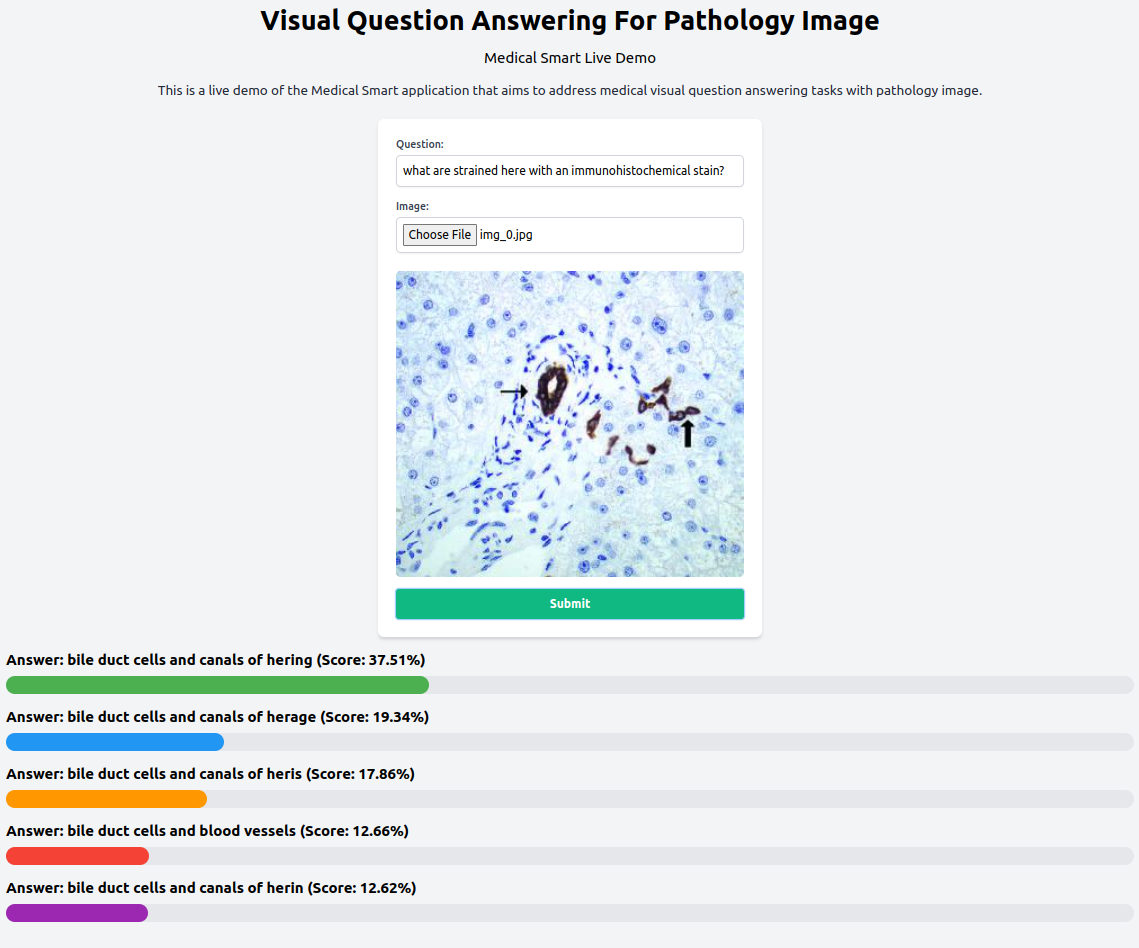
\includegraphics[width=\textwidth, height=10cm]{image/lampiran/patologi-1.png}
  \end{figure}

  \begin{figure}[H]
    \centering
    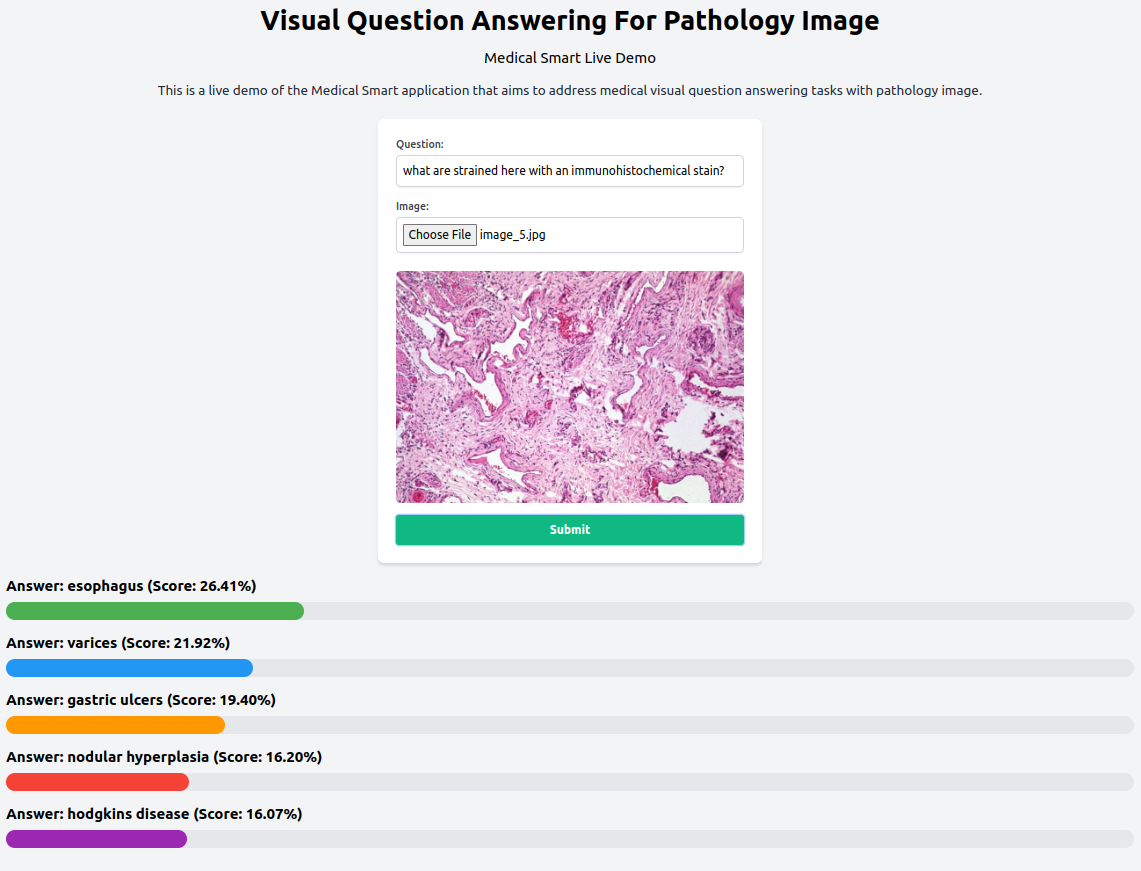
\includegraphics[width=\textwidth, height=10cm]{image/lampiran/patologi-2.png}
  \end{figure}

  \begin{figure}[H]
    \centering
    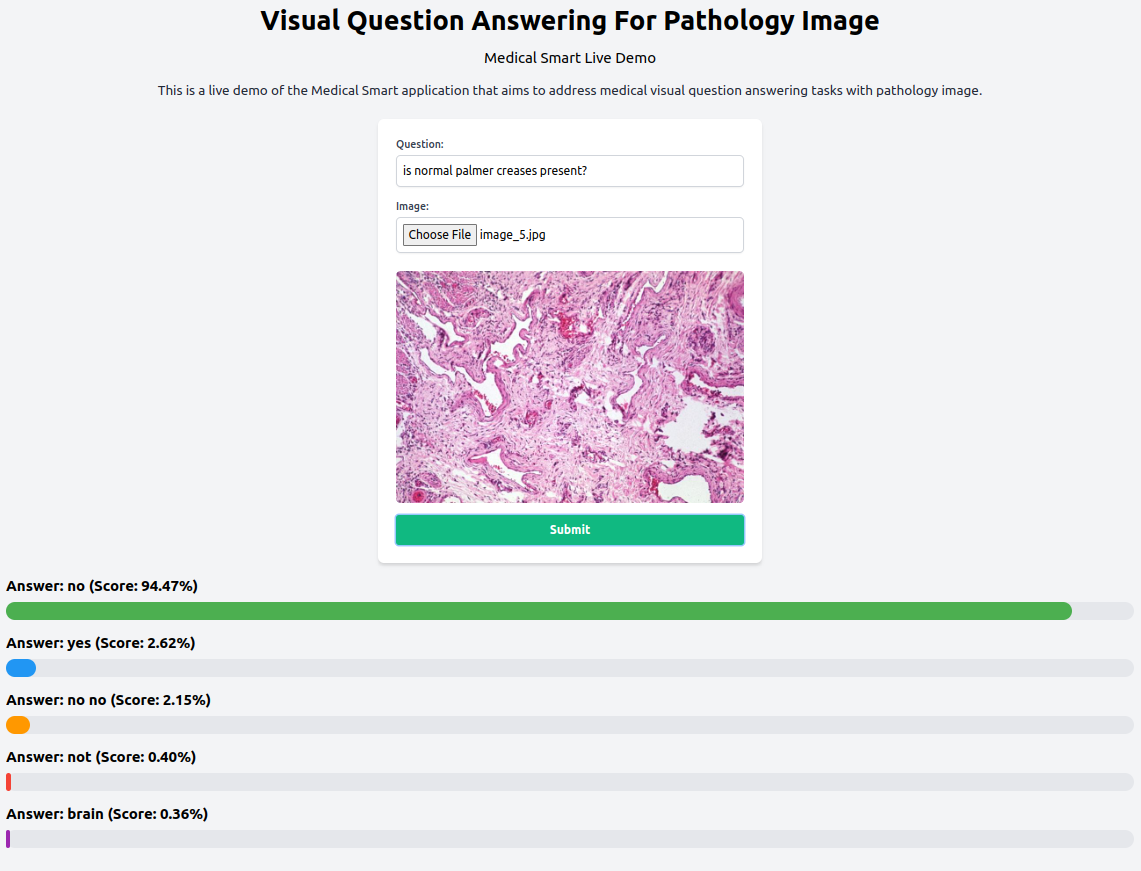
\includegraphics[width=\textwidth, height=11cm]{image/lampiran/patologi-3.png}
  \end{figure}

  \begin{figure}[H]
    \centering
    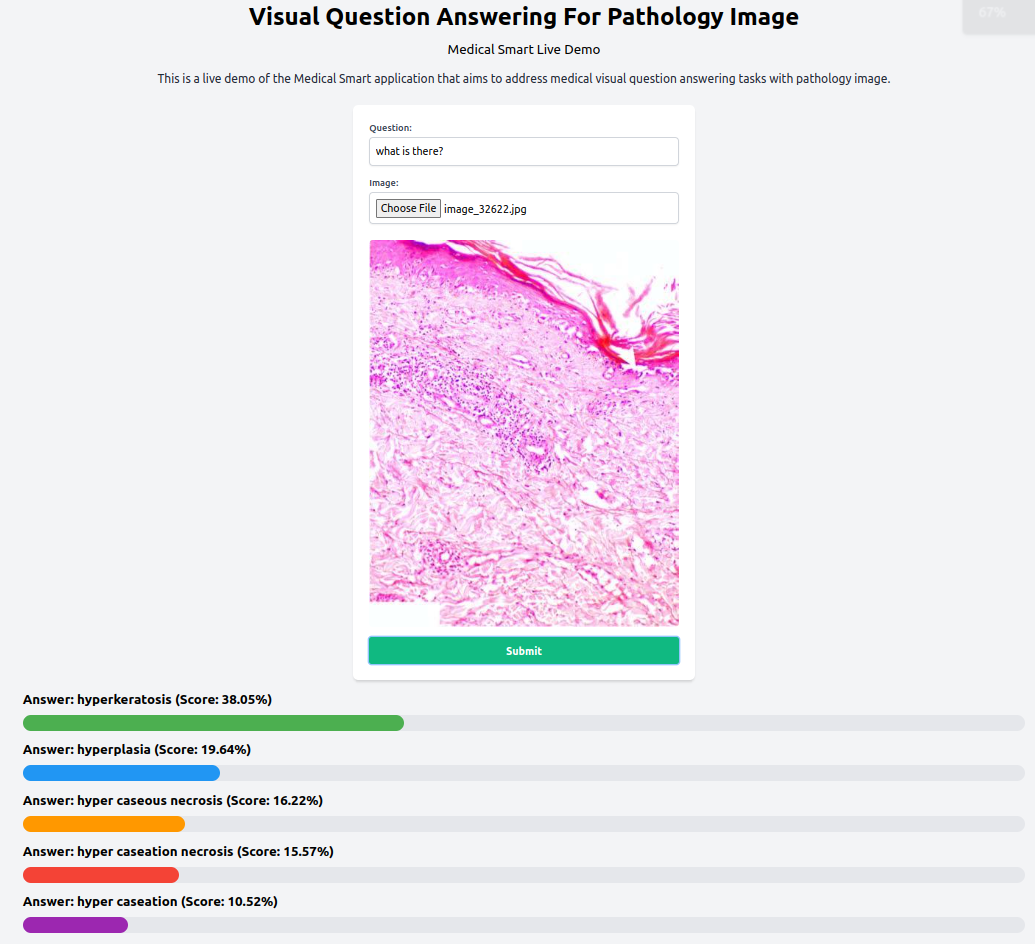
\includegraphics[width=\textwidth, height=10cm]{image/lampiran/patologi-4.png}
  \end{figure}
  

  \newappendix{Lampiran 11. Proses demo pada citra radiologi di halaman web}

  \begin{figure}[H]
    \centering
    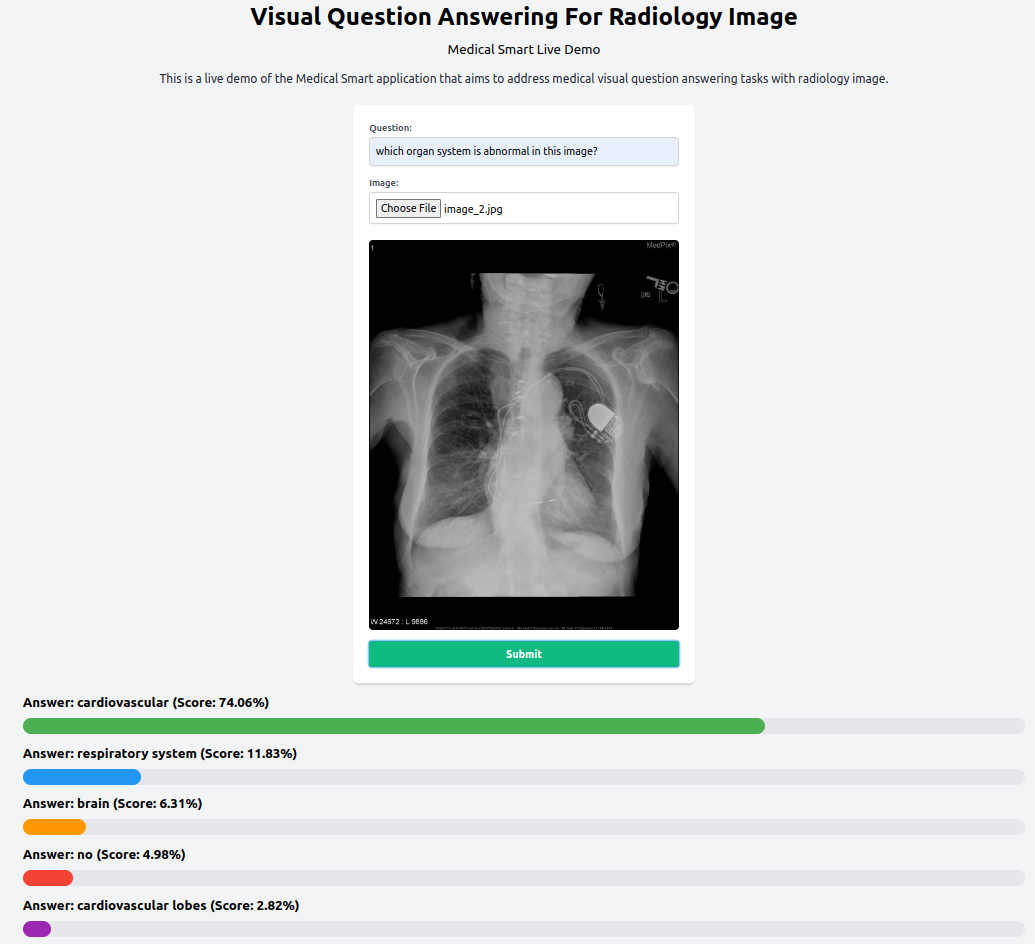
\includegraphics[width=\textwidth, height=10cm]{image/lampiran/radiologi-1.png}
  \end{figure}

  \begin{figure}[H]
    \centering
    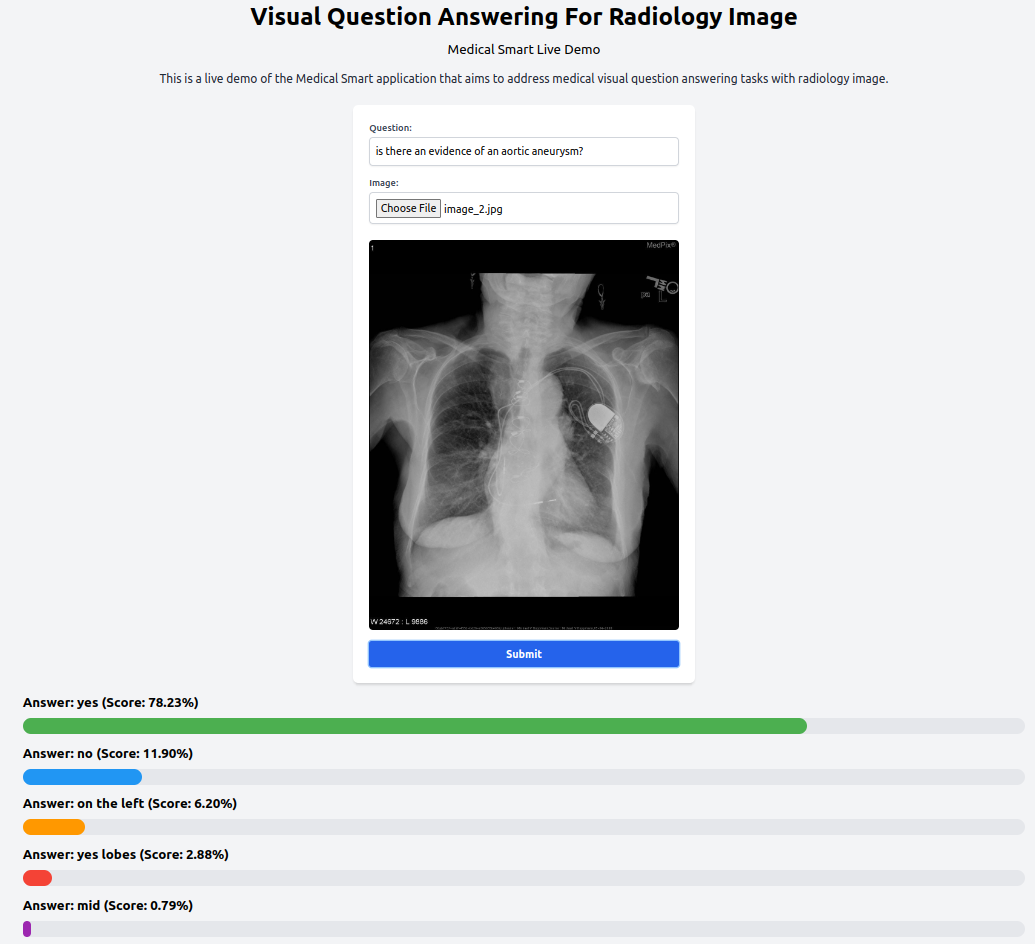
\includegraphics[width=\textwidth, height=11cm]{image/lampiran/radiologi-2.png}
  \end{figure}

  \begin{figure}[H]
    \centering
    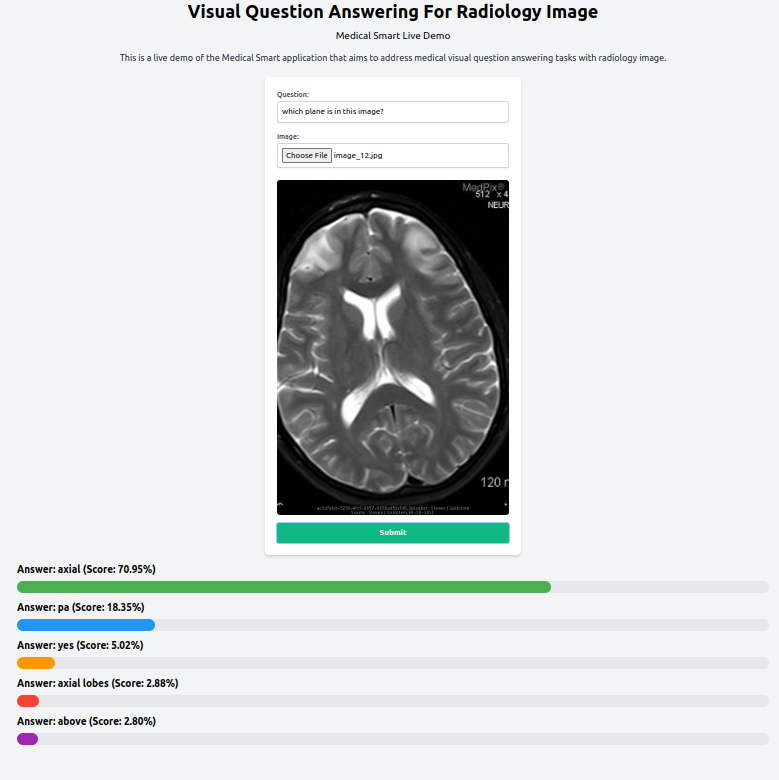
\includegraphics[width=\textwidth, height=11cm]{image/lampiran/radiologi-3.png}
  \end{figure}

  \begin{figure}[H]
    \centering
    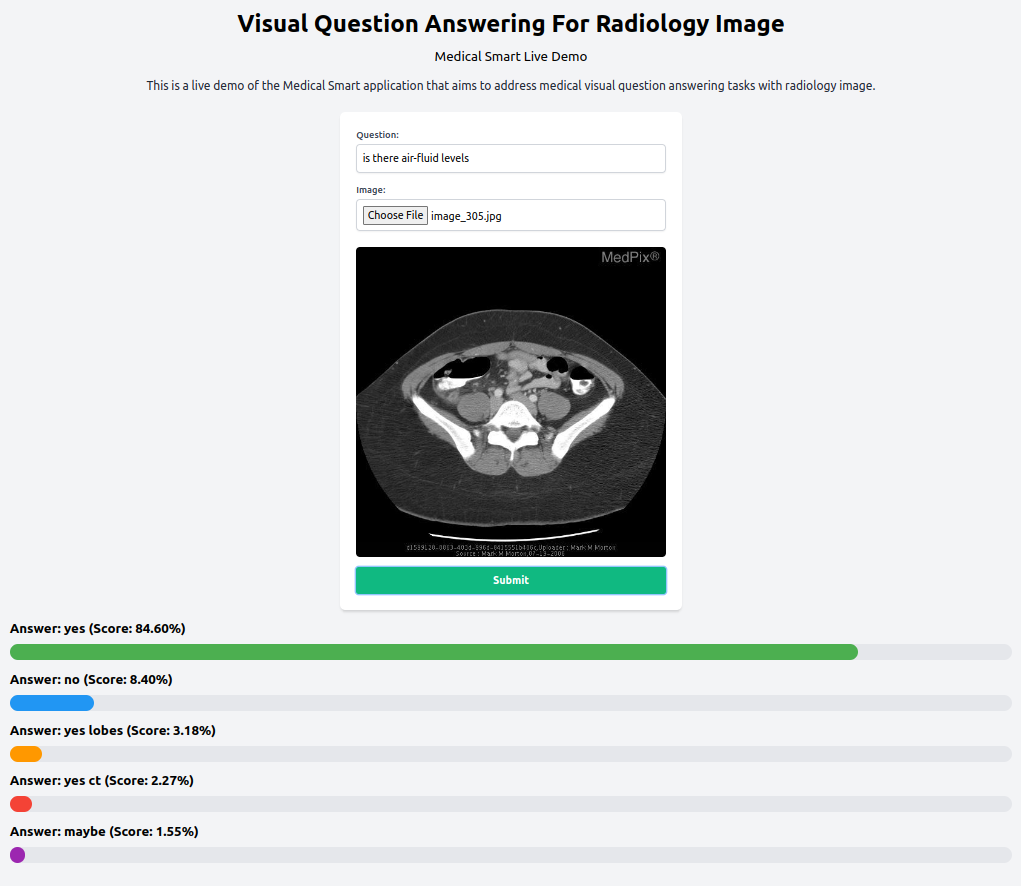
\includegraphics[width=\textwidth, height=11cm]{image/lampiran/radiologi-4.png}
  \end{figure}

  \newappendix{Lampiran 12. Biodata Penulis}

  %\includepdf[pages=-]{tanda-tangan/biodata-signed.pdf} --> Jika sudah ada tanda tangan, komen code bawah dan uncomment code ini

  % space kebawah 1 spasi
  \bigskip
  \vspace{1sp}
  % teks dengan font 14 ke tengah
  \begin{center}
      \fontsize{14}{16}\selectfont
      \textup{\textbf{BIODATA}}
  \end{center}
  % space kebawah 2 spasi
  \vspace{2sp}

  \begin{tabbing}
    \hspace{2in} \= \hspace{2in} \kill
    1. Nama \> : Abdul Hafidh \\
    2. Tempat, tanggal lahir \> : Banda Aceh, 29 Maret 2002 \\
    3. Alamat \> : Jalan Pari No 49 Lampriet Banda Aceh \\
    4. Nama Ayah \> : Fadhli \\
    5. Pekerjaan Ayah \> : Swasta \\
    6. Nama Ibu \> : Dewi Ratna Sari \\
    7. Pekerjaan Ibu \> : Pegawai Negeri Sipil \\
    8. Alamat Orang Tua \> : Jalan Pari No 49 Lampriet Banda Aceh \\
    9. Riwayat Pendidikan \> : 
  \end{tabbing}

  \begin{table}[H]
  \centering
  \resizebox{\textwidth}{!}{%
  \begin{tabular}{|c|c|c|c|c|}
  \hline
  \multicolumn{1}{|l|}{Jenjang} & \multicolumn{1}{l|}{Nama Sekolah} & \multicolumn{1}{l|}{Bidang Studi} & \multicolumn{1}{l|}{Tempat} & \multicolumn{1}{l|}{Tahun Ijazah} \\ \hline
  SD  & SD Kartika XIV-1 Banda Aceh     & -   & Banda Aceh & 2014 \\ \hline
  SMP & SMP Fatih Bilingual School Banda Aceh & -   & Banda Aceh & 2017 \\ \hline
  SMA & SMA Fatih Bilingual School Banda Aceh & IPA & Banda Aceh & 2020 \\ \hline
  \end{tabular}%
  }
  \end{table}


  \begin{tabular}{p{7.5cm}l}
    &Banda Aceh, 8 Juli 2024\\
    &\\
    &\\
    &\multirow{1.5}{7.5cm}{\underline{Abdul Hafidh}} \\ 
    &NPM. 2008107010056 \\
  \end{tabular}

      